%!TEX encoding = UTF-8 Unicode  
\chapter{引言}
 在实际工程计算中,尤其是在微分方程数值解、线性规划等的有限元分析中,经常出现高阶的矩阵运算,经常出现百万阶、千万阶的矩阵运算,而如果使用全矩阵运算,假设是百万阶的float类型的矩阵,则需要$4*10^{12}B$来存储,也就是4TB的空间,这显然是无法被微型计算机甚至是工作站所接受的。但是通常这些矩阵具有稀疏的性质,拥有着大量的零元,而且通常阶数越高稀疏度越高。这就可以在相当大的程度上减少了存储对于硬件的压力。同时,在计算中,大量对于0的运算是无谓的消耗资源的操作,也可以利用稀疏矩阵来避免这些无谓的操作。而在本研究中编写的稀疏矩阵库可以用来方便快捷的实现稀疏矩阵的存储以及一些基本运算,避免了使用者大量编写存储底层的代码,提高开发效率。


\chapter{研究背景综述}
近年来,在工程应用中,求解高阶矩阵的需求日益增长,全矩阵运算脱离了实际的硬件限制,为了满足这一日益增长的需求,同时这些矩阵通常都有着一个特征——非零元远少于零元,稀疏矩阵这门学科便应运而生。
在 20 世纪 60 年代研发电子网络的电子工程师们是最早的去利用稀疏性来应用稀疏矩阵进行工程上的计算的。
\cite{YousefSaad2003applied}

而在微分方程数值解、线性规划等的有限元分析中,经常出现求解高阶稀疏线性方程组,如利用全矩阵进行存储,则需要$n^2$的空间复杂度和$n^3$的乘法运算时间复杂度,显然,这种程度的运算量是无法被微型计算机,甚至是工作站所接受的。
而利用矩阵的稀疏性,可以有效地减小消耗很多无谓的存储空间以及无谓的计算,在很大的程度上降低了时间和空间复杂度,降低了计算对硬件的需求,使计算成为可能。


\section{稀疏矩阵的定义}
稀疏矩阵是非零元远小于矩阵元素总数,且非零元分布没有规律的矩阵。
\cite{YousefSaad2003applied}

\section{稀疏矩阵已有存储方式}
在这些年的发展中,出现了很多的存储方法,比如:对角线存贮法、对称矩阵的变带宽存贮法、坐标存贮法、Elipack-Itpack存贮法、CSR存贮法、Shermans存贮法、超矩阵存贮法、动态存贮方案等。\cite{sparseMatrixTech2006Zhangsun}

\subsection{三元组(Triplet)存储}
顾名思义,三元组存储方法就是分别存储矩阵的非零元所在的行列索引值,以及与之对应的非零元的值的存储方案。\cite{fengguangxiang2010.}
\newline
三元组存储方案有着直观、易于实现、顺序无关的特性,但是与传统的存储方法一样,三元组存储方案不便于求解算法的使用,不利于利用矩阵的稀疏性。
典型的C语言实现为\newline
\begin{lstlisting}

struct triplet_matrix{ 
	int *Ti;/*row pointer*/ 
	int *Tj;/*column pointer*/
	double *Tx;/*value pointer*/
	int Tnz;/*number of entries*/
	int Tnrow;/*number of rows*/
	int Tncol;/*number of columns*/
};

\end{lstlisting}
下面对应于矩阵的三元组存储:
\newline\newline\newline\newline\newline
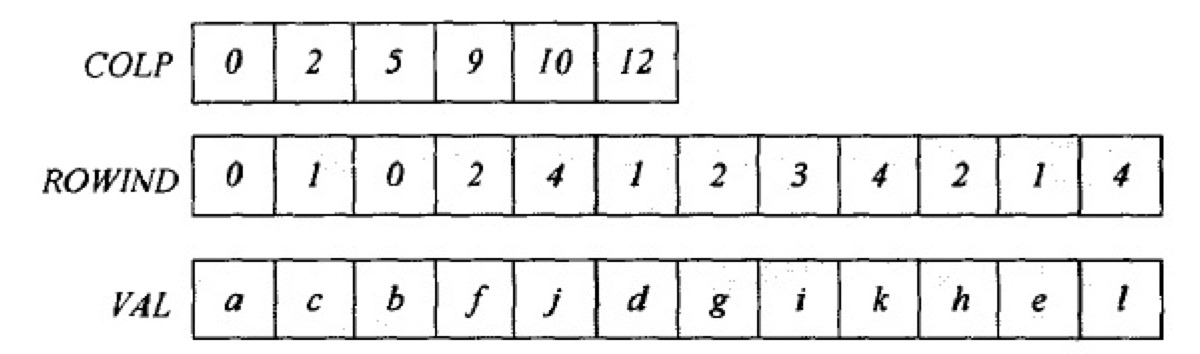
\includegraphics[scale=0.25]{triplet.png}

\subsection{十字链表(Orthogonal List)存储}
稀疏矩阵可以用上述的三元组存储方式存储,但是当稀疏矩阵的非零元的位置或个数经常变化时,使用三元组存储方式就效率低下,而十字链表法能有效的提高存取效率。十字链表法不仅为稀疏矩阵的每一行设置一个单独的行循环链表,而且同样为每一列设置一个单独的列循环链表。因此,每一个非零元同时存在于两个链表中,即包含它们的行循环链表和列循环链表,亦即这两个链表的交汇处。\newline
稀疏矩阵的链表节点需要同时存储所在的行号(row)、列号(col)、相应的元素值(value)、向下指针(down)、向右指针(right)。典型的C语言结构实现为:
\begin{lstlisting}
typedef struct node {
    int row, col;
    union {
        int val;
        struct node *ptr;
    };             //value域包括两种类型
    struct node *right, *down;
}CNode, *CrossLink;
\end{lstlisting}
\subsection{列压缩CSS(Compressed-column storage)存储}
任何矩阵的运算都涉及到矩阵的存储与读取操作,因此,存取效率对于矩阵运算的效率有着极大的影响。\newline
许多开源库采用了该存储结构,如UMFPACK、TAUCS等。列压缩存储方案较前面的三元组存储方案较不好理解,但是在矩阵计算中能更为高效地利用矩阵的稀疏性,而这也就是各大求解器采用这一存储方案的原因。\cite{fengguangxiang2010.}
\newline
列压缩存储维护了三组数据——(各列非零元的累加值,按递增的顺序存储的每列的非零元的行索引值,对应第二组数据行索引值位置对应的非零元的值)。
典型的C语言结构实现为\newline
\begin{lstlisting}

struct cc_matrix{ 
	int *Ai;/*row index*/ 
	int *Ap;/*length ncol+1*/
	double *Ax;
	
	int Ancol;
	int Anrow;
};

\end{lstlisting}
下面对应于矩阵的列压缩存储:
\newline\newline\newline\newline\newline
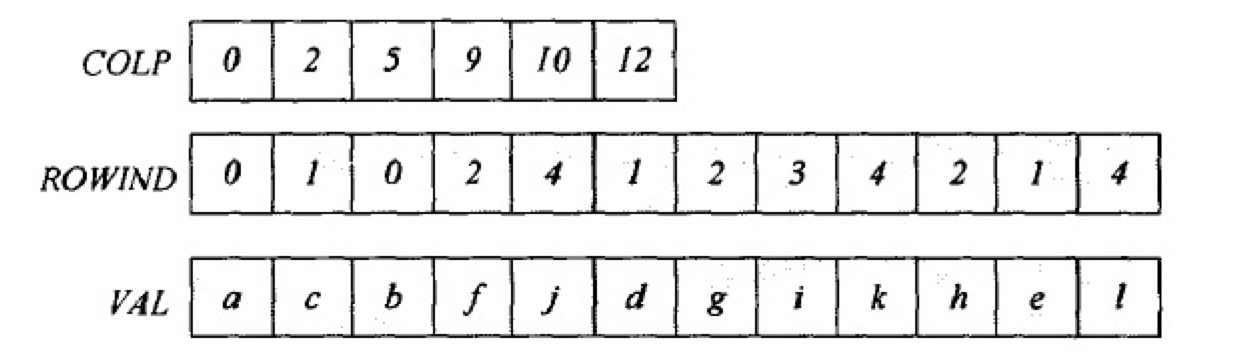
\includegraphics[scale=0.25]{ccmatrix.png}

\subsection{行压缩存储方式(Compressed Row Storage)}

CRS存储可以高效地存取任意一行非零元素,但存取任意一列非零元则需要遍历整个CRS存储结构。相应地,与CRS存储的稀疏矩阵相关的算法要高效的编程实现,算法的计算顺序必须按行来进行。\cite{fengguangxiang2010.}
下面对应于CRS存储:
\newline\newline\newline

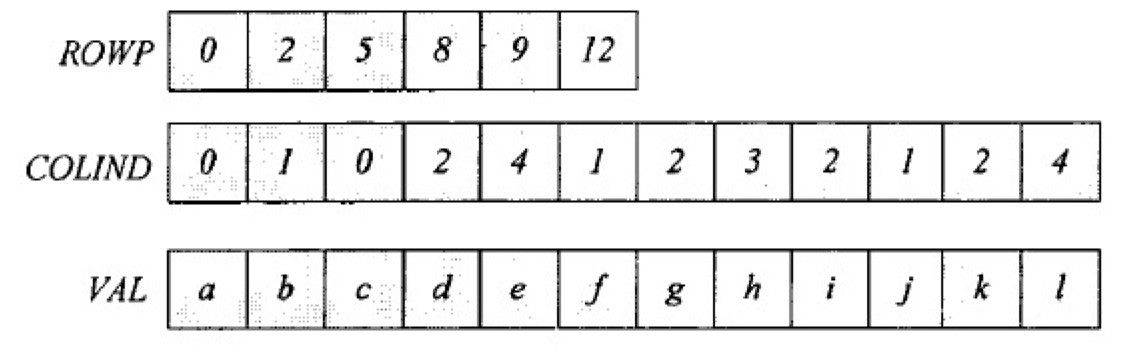
\includegraphics[scale=0.25]{crs.png}
\newline\newline
我们可以发现,ROWP数组存储的时行非零元的增长量。COLIND则存储的是列索引值,典型的C语言结构实现为\newline

\begin{lstlisting}

struct cr_matrix{ 
	int *Ri;/*col index*/ 
	int *Rp;/*length nrow+1*/ 
	double *Rx; 
	int Rncol;
	int Rnrow;
};

\end{lstlisting}

显然,越是简单的数据结构,存取操作的效率越高,亦即寻址操作的效率越高。例如,传统的稠密矩阵的存储方案只需根据行列索引值即可计算得到数据所在的地址,轻松高效的实现存取操作。在列压缩存储的稀疏矩阵中,显然能高效地存取矩阵的一列,但是,存取行的效率是极为低下的。因此,在矩阵的运算中,我们希望能尽可能地按列进行,而不是按行进行。CRS存储可以高效地存取任意一行非零元素,但存取任意一列非零元则需要遍历整个CRS存储结构。相应地,与CRS存储的稀疏矩阵相关的算法要高效的编程实现,算法的计算顺序必须按行来进行。\cite{fengguangxiang2010.}
下面对应于CRS存储:
\newline\newline\newline

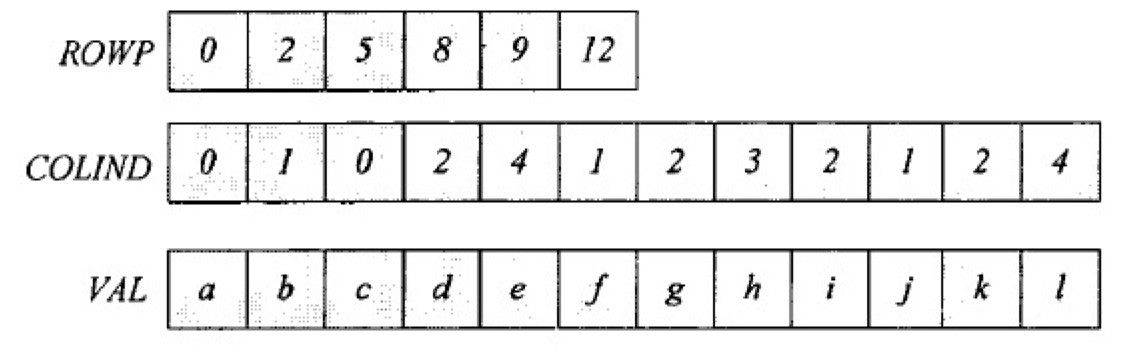
\includegraphics[scale=0.25]{crs.png}
\newline\newline
我们可以发现,ROWP数组存储的时行非零元的增长量。COLIND则存储的是列索引值,典型的C语言结构实现为\newline

\begin{lstlisting}

struct cr_matrix{ 
	int *Ri;/*col index*/ 
	int *Rp;/*length nrow+1*/ 
	double *Rx; 
	int Rncol;
	int Rnrow;
};

\end{lstlisting}

显然,越是简单的数据结构,存取操作的效率越高,亦即寻址操作的效率越高。例如,传统的稠密矩阵的存储方案只需根据行列索引值即可计算得到数据所在的地址,轻松高效的实现存取操作。在列压缩存储的稀疏矩阵中,显然能高效地存取矩阵的一列,但是,存取行的效率是极为低下的。因此,在矩阵的运算中,我们希望能尽可能地按列进行,而不是按行进行。

\section{已有的处理稀疏矩阵存储与运算的开源库}

在做稀疏矩阵的计算时,通常都是做一系列的基本运算,如:矩阵转置、矩阵向量乘法、矩阵矩阵乘法、数乘等。为了能得到更好的效率,许多研究者致力于寻找对于这些计算最优的存储结构及计算算法,同时提供了许多类库供科学计算使用,如:Portable, ExtensibleToolkit for Scientific Computation(PETSc)、Boost、GNU Scientific Library (GSL)等。\newline
例如,在Boost-uBLAS中有着稀疏矩阵的模板mapped\_matrix<T, F, A>(元素映射矩阵存储形式)、compressed\_matrix<T, F, IB, IA, TA>(压缩存储格式)、coordinat\_matrix<T, F, IB, IA, TA>(坐标存储格式)。
分别有着如下示例:\cite{boost_ublas}\newline
\textbf{mapped\_matrix:}
\begin{lstlisting}

#include <boost/numeric/ublas/matrix_sparse.hpp>
#include <boost/numeric/ublas/io.hpp>

int main () {
    using namespace boost::numeric::ublas;
    mapped_matrix<double> m (3, 3, 3 * 3);
    for (unsigned i = 0; i < m.size1 (); ++ i)
        for (unsigned j = 0; j < m.size2 (); ++ j)
            m (i, j) = 3 * i + j;
    std::cout << m << std::endl;
}

\end{lstlisting}

\textbf{compressed\_matrix:}
\begin{lstlisting}

#include <boost/numeric/ublas/matrix_sparse.hpp>
#include <boost/numeric/ublas/io.hpp>

int main () {
    using namespace boost::numeric::ublas;
    compressed_matrix<double> m (3, 3, 3 * 3);
    for (unsigned i = 0; i < m.size1 (); ++ i)
        for (unsigned j = 0; j < m.size2 (); ++ j)
            m (i, j) = 3 * i + j;
    std::cout << m << std::endl;
}

\end{lstlisting}

\textbf{coordinate\_matrix:}
\begin{lstlisting}

#include <boost/numeric/ublas/matrix_sparse.hpp>
#include <boost/numeric/ublas/io.hpp>

int main () {
    using namespace boost::numeric::ublas;
    coordinate_matrix<double> m (3, 3, 3 * 3);
    for (unsigned i = 0; i < m.size1 (); ++ i)
        for (unsigned j = 0; j < m.size2 (); ++ j)
            m (i, j) = 3 * i + j;
    std::cout << m << std::endl;
}
\end{lstlisting}

\section{稀疏矩阵的数乘}
根据数乘的定义,若矩阵A的=\{$a_{ij}$\},则kA=\{$ka_{ij}$\},则稀疏矩阵的数乘可以简单的定义为所有非零元乘上这个数。例如:对(1)实现的三元组存储的稀疏矩阵的数乘可以用如下函数进行计算:
\begin{lstlisting}
void multi(triplet_matrix matrix,double k){
	for(int i=0;i<Tnz;i++){
		*Tx[i]=*Tx[i]*k;
	}
}
\end{lstlisting}

\section{稀疏矩阵的矩阵向量乘法}
根据矩阵向量乘法的定义:
$$
\left (                 
\begin{array}{cccc}   
    a_{11} & a_{12}& \cdots & a_{1n}\\  
    a_{21} & a_{22}& \cdots & a_{2n}\\  
     \vdots & \vdots& \ddots  & \vdots \\ 
    a_{n1} & a_{n2}& \cdots & a_{nn}\\     
\end{array}
\right)          
\left (                 
\begin{array}{c}   
    b_{1} \\  
    b_{2} \\  
    \vdots \\  
    b_{n} \\  
\end{array}
\right)           
=
\left (                 
\begin{array}{c}   
    a_{11}b_{1}+ a_{12}b_{2}+\cdots+a_{1n}b_{n}\\  
    a_{21}b_{1}+ a_{22}b_{2}+\cdots+a_{2n}b_{n}\\  
    \vdots \\  
     a_{n1}b_{1}+ a_{n2}b_{2}+\cdots+a_{nn}b_{n}\\  
\end{array}
\right)   
$$
由于零元参与运算对计算结果没有影响,所以在计算中可以不对零元计算,亦即在稀疏矩阵的矩阵向量运算中,可以只对非零元进行计算。亦即对A的每一列j的非零元$a_{ij}$执行
$$z_i=y_i+a_{ij}x_j$$

那么,我们可以很方便的利用矩阵的稀疏性对列压缩存储的稀疏矩阵进行上述操作,示例代码如下
\begin{lstlisting}
for(int j=0;j<Ancol;j++){
	for(int p=Ap[j];p<Ap[j+1];p++){
		z[Ai[p]]=Ax[p]*x[j]+y[Ai[p]];
	}
}
\end{lstlisting}



\section{稀疏矩阵的矩阵矩阵乘法}
根据矩阵向量乘法的定义:
$$
\left (                 
\begin{array}{cccc}   
    a_{11} & a_{12}& \cdots & a_{1n}\\  
    a_{21} & a_{22}& \cdots & a_{2n}\\  
     \vdots & \vdots& \ddots  & \vdots \\ 
    a_{n1} & a_{n2}& \cdots & a_{nn}\\     
\end{array}
\right)          
\left (                 
\begin{array}{cccc}   
     b_{11} & b_{12}& \cdots & b_{1n}\\  
    b_{21} & b_{22}& \cdots & b_{2n}\\  
     \vdots & \vdots& \ddots  & \vdots \\ 
    b_{n1} & b_{n2}& \cdots & b_{nn}\\ 
    \end{array}
\right)           
=
\left (                 
\begin{array}{cccc}   
     c_{11} & c_{12}& \cdots & c_{1n}\\  
    c_{21} & c_{22}& \cdots & c_{2n}\\  
     \vdots & \vdots& \ddots  & \vdots and\\ 
    c_{n1} & c_{n2}& \cdots & c_{nn}\\ 
\end{array}
\right)   
$$
其中,对于任意的i,j,有$$
c_{ij}=\sum_{k=1}^na_{ik}b_{kj}
$$
由于零元参与运算无意义,在计算中可以将零元不进行运算。
亦即$$
c_{ij}=\sum_{k=1,a_{ik}\neq 0,b_{kj} \neq 0}^na_{ik}b_{kj}
$$

